\section{Who loses a placement?}\label{sec:who}
At the level of a whole market, both studies give instances of higher coverage and fewer placements. The losses reach different people. Figure~\ref{fig:losses} partitions everyone who was placed under $A$ and unplaced under $B$. We first separate people whose menu was identical. Among the rest, we ask whether their full-list partner became visible, became hidden, or had the same visibility as before.

\begin{figure}[ht]
\centering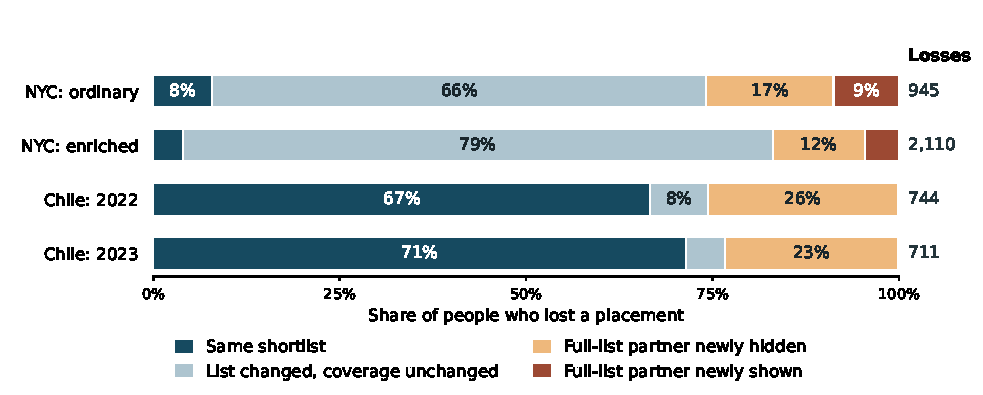
\includegraphics[width=.97\linewidth]{figures/placement-losses.pdf}
\caption{What changed for people who lost a placement? Bars within each row sum to 100\%. Numbers at right are raw gross losses. A changed list can retain the same partner coverage, including when the applicant had no full-list partner. The latter applicants still count in the analysis.}
\Description{The share of placement losses on an identical menu is small in the rental simulation, and about seven in ten in both Chilean school cohorts.}
\label{fig:losses}
\end{figure}

\paragraph{A change that reaches someone else's list.}
In the original 2022--23 Chilean cohorts, only 32,914 of 1,107,244 application records had different displayed courses under the two predictors. Of 1,455 applicants who lost a placement, 1,004 had exactly the same personal menu. The reverse happened to 406 of the 470 who gained one. Holding preferences, priorities, capacities and an applicant's own list fixed, a change in that applicant's placement can arise only through competitors' menus. These spillovers account for a net loss of 598 seats among applicants whose lists stayed fixed. Among the 32,914 applicants with edited lists, 451 lost a place (1.37\%). Among the 1,074,330 with identical lists, the 1,004 losses represent 0.093\%.

In the ordinary NYC markets, 945 renter instances lost a placement and 475 gained one. Of the 945 who lost, 74 saw identical menus and 83 newly saw their full-list partner. In enriched markets, 2,110 lost a placement and 1,212 gained one. Here 83 of those who lost saw identical menus and 97 newly saw their partner. Over both designs, newly seeing one's full-list partner and losing a place happened to 180 renter instances. For all 180 we found the distinct displaced-partner witnesses in Theorem~\ref{thm:two-omission} within their respective market. Of these paths 169 reached a witness after one program. Longer paths involved up to three programs.

\paragraph{The newly shown school offer often converted.}
In Chile in 2022--23, 3,750 applicants newly saw their full-list DA partner under the rank-informed predictor. Of these, 3,728 obtained that exact course in the replay and 20 obtained a different course. The remaining two went unplaced. In ordinary NYC markets 1,056 of the 1,720 newly shown renters obtained the named apartment (61.4\%); in enriched markets it was 1,277 of 2,012 (63.5\%). Across all applicants in each NYC design the number receiving their exact full-list partner increased by 523 and 553, respectively. Across the two school cohorts it increased by 5,049. More people therefore received their exact full-list partner even while fewer received any placement. We verified both displacement paths. Analyzing the recorded historical offer as a separate target, 3,366 of the 3,622 applicants who newly saw that program received it in the replay. Thus a platform could document a high rate of placement at the newly shown program and still miss a loss elsewhere in the market. The witness theorem applies to the modeled full-list partner. It uses stability and cannot be applied to an arbitrary historical offer.

\paragraph{Feasibility and priorities.}
Let $\nu(D)$ be the largest number who can simultaneously take displayed options within capacity, and $g(D)=\nu(D)-|N_D|$ the feasible places unrealized by DA. The placement change is $\Delta\nu-\Delta g$ \citep{aguiarhong2026}. In ordinary NYC markets, displayed capacity fell by 3.84 percentage points and the shortfall shrank by 1.13, giving the observed 2.71-point decline. In enriched markets those changes were $-12.29$ and $-6.89$ points. The school results differ. In 2022 the display could accommodate 244 fewer applicants and the shortfall grew by 224, for a loss of 468. In 2023 those figures were 153 and 364, for a loss of 517. Each school maximum is certified by a feasible flow and a cut of equal value. This benchmark uses only displayed edges and seat counts. It relaxes priorities and the obligation to place a particular returning pupil. These identities describe two margins on the same graph. They do not isolate the causal effect of changing priorities.
